	\section*{Background and motivation}
	


	
Using popular on-line video/image retrieval engines, and running the query “apple”, provided document contents illustrate this problem (see Figure \ref{fig_intro::serach_image}). Indeed, this query term is ambiguous: it means a fruit, and also the trademark “apple”. Furthermore, in figure \ref{fig_intro::serach_video}, videos displayed as results for the same query illustrate also that search engines still using some meta-data (such as the title) to understand a video contents. Moreover, these systems are still based on the manual annotation of multimedia content. This is shown in Figure \ref{fig_intro::serach_extra} where the retrieval engine prompts the user to clearly clarify its query by suggesting extra information in connection with his request.
	
		\begin{figure}[ht!]
				\centering
				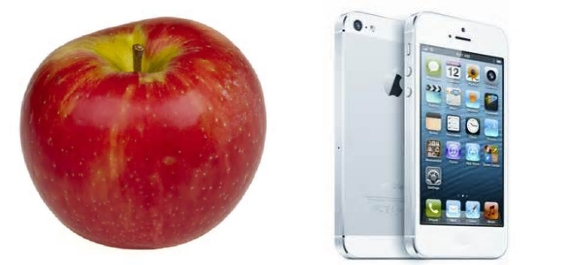
\includegraphics[width=0.4\textwidth]{figures/fig_intro::serach_image}	
				\caption{Sample Image Results from querying \textit{Yahoo!} search engine using the term \textit{"apple"}}
				\label{fig_intro::serach_image}
			\end{figure}
			\begin{figure}[ht!]
					\centering
					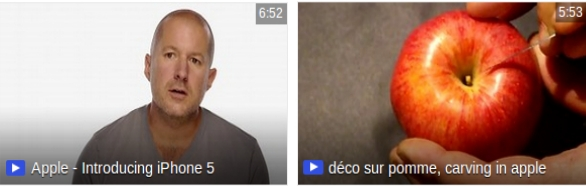
\includegraphics[width=0.6\textwidth]{figures/fig_intro::serach_video}
					\caption{Sample Video Results from querying \textit{Yahoo!} search engine using the term \textit{"apple"}}
					\label{fig_intro::serach_video}
			\end{figure}
			\begin{figure}[ht!]
					\centering
					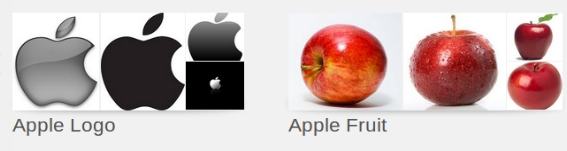
\includegraphics[width=0.6\textwidth]{figures/fig_intro::serach_extra}
					\caption{The Google retrieval engine prompts the user to further define its query}
					\label{fig_intro::serach_extra}
			\end{figure}
	
	Although these multimedia research systems still suffer from many limitations as mentioned above, they are in wide use by all users. Indeed, these systems rely primarily on the response time rather than on the relevance efficiency of provided documents.
	
	Modeling multimedia retrieval systems has motivated many researchers, in particular in the last decade. These efforts have led to a variety of methods and models based on the semantic indexing (interpretation) of a multimedia content. These latter are commonly based on a standard model that continues to grow and to getting efficient. Indeed, early works was focused on low-level features (that are related essentially on the analysis of color and brightness). This work quickly shown its limits where two different non similar contents can show the same color and brightness repartition (the semantic gap). This gap forced researchers to index the semantic content by identifying objects (called also concept) and use them to find similar contents. Concept detection was based on a learning algorithm. A manual annotation process on a multimedia dataset is used for that algorithm. Concept-based multimedia retrieval models lead to spectacular results, but they raised new problems: a detected object can be ambiguous, and the context in what it's defined have to be stated too.
	
	Summarizing, and analyzing these semantic multimedia indexing models, we observe that the low-level features, concepts and contexts based models look for describing what exists in a content. However, in analogy with a human interpretation, a multimedia content interpretation is based both on the detection and the analysis of present objects, and also on a reasoning process which deals with knowledge-background.
	
	In reality, supporting higher-level of an automated conceptual understanding and reasoning has been introduced in the IR area since the late nineties with the emergence of the Semantic Web. The latter aims to enable a machine to automatically find, understand, combine and share information about a resource (a document) efficiently. Actually, ontologies are considered as key element to handle knowledge and to overcome existent IR system problems. Their potential was envisaged and explored in many recent research works. Yet, Ontology-based model are widely considered in IR community, but it's still great deal of effort to spend in this line of research.
	
	\paragraph{Multimedia Indexing Challenges}
	
	Earlier proposed approaches for bridging the semantic gap was centered on exploring low-level features in order to detect potential semantic concepts. These approaches rely on some rules that maps these low-level features to concepts. But it was very difficult to benchmark their efficiency because every approach is evaluated on very closed datasets. Then, it was a very pressing challenge for researchers to judge if their approaches are promising or not. Indeed, and regarding strong copyrights to access and share a large amount of multimedia data, it was very hard to create and share a common shared multimedia dataset.
	
	In order to overcome this obstacle, The NIST(the \textit{American National Institute of Standards and Technology}) initiated the TRECVID \cite{phd::Smeaton2001,phd::Oomen2013}(\textit{TREC Video Retrieval Evaluation}) in order to deliver a common benchmark framework to the Multimedia Retrieval community. This framework consisted in a common large digital video dataset, common metrics for the evaluation and some tasks including motion detection, story segmentation, semantic indexing, \dots. Then, researchers rapidly adopted this evaluation campaign by evaluating their algorithm and sharing their results.
	
	Through this evaluation campaign, detecting semantic concepts by mapping some low-level features showed its limits \cite{Snoek2006}. In fact, this approach can be applied on a very limited concept set, and it's very hard to define particular low-level features aggregation for large number of concepts. So, another challenge pressed the Multimedia Retrieval community. The latter migrated to a generic concept detection through machine learning approach. To cope with this trend, many shared collaborative multimedia annotated datasets have been proposed \cite{phd::Lin2003, phd::Volkmer2005a, phd::Ayache2007a, phd::Huiskes2008, Thomee2012}. These datasets helped researchers to learn their system how to detect concepts.
	
	First evaluation campaigns proposed the detection of a restricted number of semantic concepts. Gradually, the number continues to increase (500 concepts in TRECVID 2013 and 116 concepts for ImageCLEF 2013 \cite{phd::Villegas2012}). Indeed, handling more multimedia data including many areas enrich the amount of handled objects then semantic concepts. However, It was very hard to researchers to develop systems able to detect this amount of concepts: In fact, some concepts are not easy to detect without the analysis of other semantic objects in interaction within the same content. Indeed, the concept “airplane\_{}flying” can be found when there are a “plane” and the “sky” in background. 	Thereby, analyzing contextual informations and concepts interrelationships is considered as a solution for enhancing learning based multimedia indexing approaches. 
	
	But again, new challenges raised: At first, (1) how the contexts in which semantic concepts are defined could be detected? (2) And how the semantic relationships between concepts could be extracted? Then (3) how to use these contexts and relationships to improve the multimedia indexing efficiency? 
	
	Recently, knowledge bases, and particularly ontologies, attracted much attention from researchers in order to deal with these inquiring. Although there where many efforts for handling knowledge databases in Multimedia Indexing field, the use of an ontology has a number of challenges: (4) what conceptual structure for that ontology ? (5) how gather new knowledge, (6) how to infer new Knowledge, (7) how to evolve its content.
	
	For example, the ontology LSCOM \cite{phd::Naphade2006} (Large Scale Concept Ontology for Multimedia) still considered as a taxonomy of a set of concepts rather than a concrete knowledge database. Moreover, other recent works focused on defining ontologies for different use  (\cite{phd::Karkaletsis2005,phd::Li2007, Zhai2008, phd::Mitschick2010a, phd::Kumar2012}). But there were not a generic ontology model for multimedia indexing.
	
	In conclusion, ontologies are promising tools to conceptualize concepts, contexts and their relationships. But some challenges related to ontologies and the very specific nature on multimedia indexing systems nature have to be addressed. In our thesis work, we detail our apprcoach to cope with these challenges.
	
	\paragraph{Aims and Contributions}
	The main goal of this thesis is to model and to integrate a fuzzy reasoning driven multimedia indexing model to support semantic indexing capabilities. Indeed, it's obvious that imprecision, vagueness and uncertainty are aspects that should be addressed in order to enhance an indexing  system performance \cite{Stoilos2005, phd::Zadeh2006}. Yet, many applications like  \cite{phd::Simou2008, phd::Elleuch2011, phd::Paliouras2011c} and many more attempted to integrate a fuzzy set theory framework in audiovisual retrieval systems \cite{phd::Zadeh1965, phd::Mendel1995, phd::Bede2013}. Expect these few research works, fuzzy knowledge management is rarely involved in multimedia area.

	Given an initial indexing of a multimedia data, our aims is to enhance such interpretation by a deep analysis based on extra knowledge. This latter has to be modeled and an inference schema has to be defined in order to show how to extend the data interpretation. 
	
	Using ontology is a common way when modeling knowledge especially in information retrieval framework []. In our context, we will adopt the same orientation but we investigate the fuzzy level. So we propose a fuzyy ontology as a knowledge structuring model. 
	
	The fuzzy aspect to be considered into an ontology content consists in defining fuzzy relationships between handled knowledge (in the form of concepts and contexts), and also a fuzzy reasoning process to generate new fuzzy knowledge from existent ones.
	
	In our proposed multimedia semantic indexing model, a fuzzy ontology will play an important role as it manages, at first, gathered semantic interpretation from multi-modal analyzers (particularly textual, audio and visual modalities), then produces enhanced interpretation through a fuzzy reasoning process.
	
	%Show that initial knowledge is deduced from elementary annotation data. 
				\begin{figure}[ht!]
					\centering
					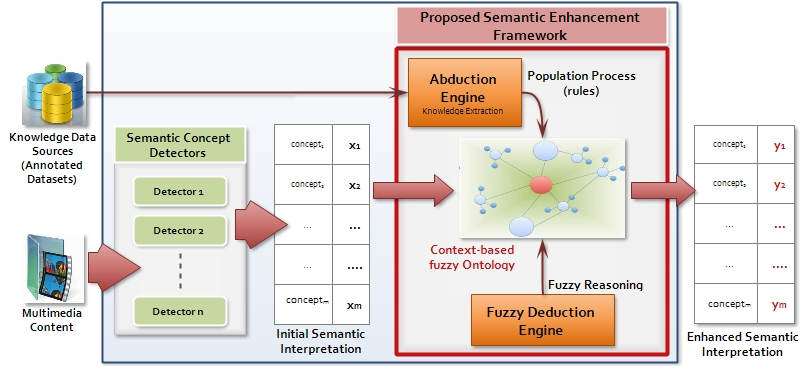
\includegraphics[width=1\textwidth]{graphics/systeme}	
					\caption{Main Contribution}
					\label{fig_intro::contribution}
				\end{figure}
	
	Within this context, the main contributions are related to the modelisation and the development of a fuzzy reasoning model. This model is based on a fuzzy knowledge database materialized by an ontology. Thus, our contribution is focused on managing a fuzzy ontology as the following points:
	
	\begin{description}
		\item[A fuzzy Ontology structure] The ontology structure reflects the conceptual level of knowledge that could be handled. Relations between data in an ontology will be modeled based on fuzzy reasoning.  
		
		\item[An Ontology Population] This level looks for identifying instances of concepts/contexts and their potential interrelationships. This step is initially performed in order to supply ontology with a knowledge background extracted from annotation results. 
		
		\item[Fuzzy Rule Inference] Rules are descriptions of particular relationships between concepts and contexts. When combined to a domain conceptualization, it can enhance and enrich the amount of knowledge in an ontology.
		
		\item[Fuzzy ontology Evolving]The ontology content should be able to answer different change requirements. The ontology content will constantly evolve according to user requirement and usage instance.
	\end{description}
	
	Then, the use of knowledge management in information retrieval systems is a stark choice for multimedia semantic indexing. Further, multimedia indexing handles documents on various topics. Our proposed model have, then, to adapt the ontology content to knowledge elicited in the collection of documents to be indexed. In this case, the generic aspect of such model should be highly addressed: the ontology content have to be gathered from data source having common knowledge background with documents being indexed. Such aspect will affect the way we model our fuzzy ontology, and in particular, how to extract and structure the conceptual knowledge.
	
	Finally, our contribution is to proposed a generic fuzzy ontology management model to be used for improving semantic multimedia indexing focusing on adaptive ability to enhance a semantic interpretation for any multimedia collection.
	
	\section*{Used approach and thesis plan}
	
The present thesis is divided into two main parts. The first part displays a general literature survey about semantic indexing systems. 
The second part exposes the proposed fuzzy ontology based model for video indexing by detailing its design, its implementation and its evaluation.

These two parts consist of individual chapters as follows:
\begin{itemize}
	\item \textbf{Part I: Context and Related Works}
		\begin{itemize}
			\item \textbf{Chapter 2 :} introduces a general overview of the Information Retrieval systems. 
								It describes also the main proposed models, the common assessment measures and the methodologies. Then, the chapter introduces a survey of the use of fuzzy knowledge databases
								to solve problems discussed in the previous chapter. 
								After enumerating actual related works, we show a discussion over the survey in order to motivate and introduce 
								our proposed fuzzy ontology based model for video indexing.
		\end{itemize}
	\item \textbf{Part II: The Fuzzy Ontology Based Model for Video Indexing}
			\begin{itemize}
			\item \textbf{Chapter 3 :} Presents our proposed model for enhancing semantic video interpretation. 
								This chapter also presents the developed framework based on our knowledge based indexing model,
			\item \textbf{Chapter 4 :} introduces a survey of the use of fuzzy knowledge databases
								to solve problems discussed in the previous chapter. 
								After enumerating actual related works, we show a discussion over the survey in order to motivate and introduce 
								our proposed fuzzy ontology based model for video indexing.
			\item \textbf{Chapter 5 :} exposed the evaluation benchmarks applied  in order to test the effectiveness 
								of our semantic indexing model. It shows finally the obtained results.
 		\end{itemize}
	\item \textbf{Chapter 6:} The final chapter displays our conclusions and contributions 
												and reveals extensions and future research lines.
\end{itemize}


